\graphicspath{{figures/quadric/}}

%\setcounter{secnumdepth}{0}
\renewcommand{\theequation}{\thechapter.\arabic{equation}}
\renewcommand{\thetheorem}{\thechapter.\arabic{theorem}}
\renewcommand{\thebc}{\thechapter.\arabic{theorem}}
\renewcommand{\theeg}{\thechapter.\arabic{theorem}}
%\counterwithin{theorem}{chapter}
%\numberwithin{theorem}{chapter}


\chapter{Conic Sections and Quadric Surfaces}\label{ap:quadric}

A conic section is the curve of intersection of a cone and a plane
that does not pass through the vertex of the cone.
This is illustrated in the figures below.
\vadjust{
\begin{efig}
\begin{center}
    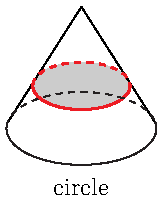
\includegraphics{conePlaneCircle.pdf}\quad
    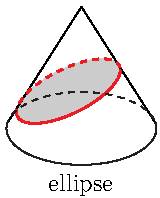
\includegraphics{conePlaneEllipse.pdf}\quad
    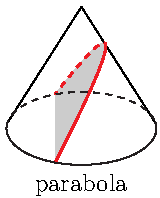
\includegraphics{conePlaneParabola.pdf}\quad
    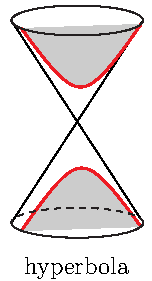
\includegraphics{conePlaneHyperbola.pdf}
\end{center}
\end{efig}
}
An equivalent\footnote{It is outside our scope to prove this equivalence.} 
(and often used) definition is that a conic section is the set of all points  
in the $xy$-plane that obey $Q(x,y)=0$ with
\begin{equation*}
Q(x,y) = Ax^2 + By^2 + Cxy + Dx + Ey + F =0
\end{equation*}
being a polynomial of degree two\footnote{Technically, we should also require
that the constants $A$, $B$, $C$, $D$, $E$, $F$, are real numbers,
that $A$, $B$, $C$ are not all zero, that $Q(x,y)=0$ has more than one 
real solution, and that the polynomial can't be factored
into the product of two polynomials of degree one.}.
By rotating and translating  our coordinate system the equation of the conic section can be brought
into one of the forms\footnote{This statement can be justified using a 
linear algebra eigenvalue/eigenvector analysis. It is 
beyond what we can cover here, but is not too difficult for a standard 
linear algeba course.}
\begin{itemize}
\item
$\al x^2 + \be y^2 =\ga$ with $\al,\be,\ga >0$, which is an ellipse
(or a circle),
\item
$\al x^2 - \be y^2 =\ga$ with $\al,\be>0$, $\ga\ne0$, which is a hyperbola,
\item 
$x^2 = \delta y$, with $\delta\ne 0$ which is a parabola.
\end{itemize}
\goodbreak

The three dimensional analogs of conic sections, surfaces 
in three dimensions given by quadratic equations, are called quadrics.
An example is the sphere $x^2+y^2+z^2=1$. Here are some tables giving
all of the quadric surfaces.

%\bigskip
\vfill
\noindent
\renewcommand{\arraystretch}{1.5}
\begin{tabular}{ | c | c | c | c | c |}
  \hline
  name & \parbox[c]{1.8cm}{\smallskip elliptic\\cylinder}
       & \parbox[c]{1.8cm}{\smallskip parabolic\\cylinder} 
       & \parbox[c]{1.8cm}{\smallskip hyperbolic\\cylinder} 
       & sphere \\[0.1in]
  \hline
  \parbox[c]{2.75cm}{\smallskip equation in\\standard form} 
             & $\frac{x^2}{a^2}+\frac{y^2}{b^2}=1$
             & $y=ax^2$ 
             & $\frac{x^2}{a^2}-\frac{y^2}{b^2}=1$
             & $x^2+y^2+z^2=r^2$\\[0.1in]
  \hline
  \parbox[c]{2.75cm}{\smallskip $x=$ constant \\cross-section} 
            & two lines 
            & one line 
            & two lines 
            & circle \\[0.1in]
  \hline
  \parbox[c]{2.75cm}{\smallskip $y=$ constant \\cross-section} 
            & two lines
            & two lines
            & two lines 
            & circle \\[0.1in]
  \hline
  \parbox[c]{2.75cm}{\smallskip $z=$ constant \\cross-section} 
            & ellipse
            & parabola 
            & hyperbola 
            & circle \\[0.1in]
  \hline
  sketch 
     & \raisebox{-45pt}[42pt][52pt]
              { \smash{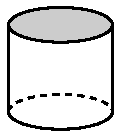
\includegraphics[scale=1.3]{cylinder.pdf}} }
     & \raisebox{-47pt}[42pt][52pt]
             {\smash{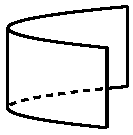
\includegraphics[scale=1.3]{parabolic_cylinder.pdf}}}
     & \raisebox{-50pt}[42pt][52pt]
             {\smash{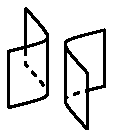
\includegraphics[scale=1.4]{hyperbolic_cylinder.pdf}}}
     & \raisebox{-47pt}[42pt][52pt]
              { \smash{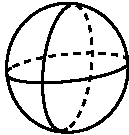
\includegraphics[scale=1.3]{sphere.pdf}} }
      \\[0.1in]
  \hline
\end{tabular}
\vfill
%\bigskip\medskip
\noindent
\begin{tabular}{ | c | c | c | c | c |}
  \hline
  name & ellipsoid 
       & \parbox[c]{1.8cm}{\smallskip elliptic\\paraboloid}
       & \parbox[c]{1.5cm}{\smallskip elliptic\\cone}  \\[0.1in]
  \hline
  \parbox[c]{2.75cm}{\smallskip equation in\\standard form} 
       & \parbox[c]{3.4cm}{\ \ \ \ 
             $\frac{x^2}{a^2}+\frac{y^2}{b^2}+\frac{z^2}{c^2}=1$} 
       & \parbox[c]{3.4cm}{\ \ \ \ \ 
             $\frac{x^2}{a^2}+\frac{y^2}{b^2}=\frac{z}{c}$}
       & \parbox[c]{2.3cm}{
             $\frac{x^2}{a^2}+\frac{y^2}{b^2}=\frac{z^2}{c^2}$} \\[0.1in]
  \hline
  \parbox[c]{2.75cm}{\smallskip $x=$ constant \\cross-section} 
            & ellipse
            & parabola
            & \parbox[c]{3.5cm}{\smallskip two lines if $x=0$\\
                                           hyperbola if $x\ne 0$}   \\[0.1in]
  \hline
  \parbox[c]{2.75cm}{\smallskip $y=$ constant \\cross-section} 
            & ellipse
            & parabola
            & \parbox[c]{3.5cm}{\smallskip two lines if $y=0$\\
                                           hyperbola if $y\ne 0$} \\[0.1in]
  \hline
  \parbox[c]{2.75cm}{\smallskip $z=$ constant \\cross-section} 
            & ellipse
            & ellipse 
            & ellipse  \\[0.1in]
  \hline
  sketch 
     & \raisebox{-50pt}[45pt][55pt]
              { \smash{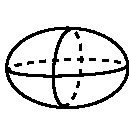
\includegraphics[scale=1.5]{ellipsoid.pdf}} }
     & \raisebox{-48pt}[45pt][55pt]
              { \smash{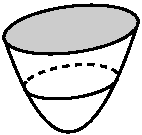
\includegraphics[scale=1.3]{elliptic_paraboloid.pdf}} }
     & \raisebox{-48pt}[45pt][55pt]
              { \smash{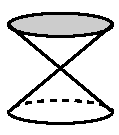
\includegraphics[scale=1.4]{cone.pdf}} }
      \\[0.1in]
  \hline
\end{tabular}
\vfill\newpage

%\bigskip\bigskip
\noindent
\begin{tabular}{ | c | c | c | c | c |}
  \hline
  name &\parbox[c]{2.75cm}{\smallskip hyperboloid\\of one sheet} 
       & \parbox[c]{2.75cm}{\smallskip hyperboloid\\of two sheets}
       & \parbox[c]{2.1cm}{\smallskip hyperbolic\\paraboloid}  \\[0.1in]
  \hline
  \parbox[c]{2.75cm}{\smallskip equation in\\standard form} 
       & \parbox[c]{3.4cm}{\ \ \ \ 
             $\frac{x^2}{a^2}+\frac{y^2}{b^2}-\frac{z^2}{c^2}=1$} 
       & \parbox[c]{3.4cm}{\ \  
             $\frac{x^2}{a^2}+\frac{y^2}{b^2}-\frac{z^2}{c^2}=-1$} 
       & \parbox[c]{2.1cm}{
             $\frac{y^2}{b^2}-\frac{x^2}{a^2}=\frac{z}{c}$} \\[0.1in]
  \hline
  \parbox[c]{2.75cm}{\smallskip $x=$ constant \\cross-section} 
            & hyperbola
            & hyperbola
            & parabola  \\[0.1in]
  \hline
  \parbox[c]{2.75cm}{\smallskip $y=$ constant \\cross-section} 
            & hyperbola
            & hyperbola
            & parabola \\[0.1in]
  \hline
  \parbox[c]{2.75cm}{\smallskip $z=$ constant \\cross-section} 
            & ellipse
            & ellipse 
            & \parbox[c]{3.5cm}{\smallskip two lines if $z=0$\\
                                           hyperbola if $z\ne 0$}  \\[0.1in]
  \hline
  sketch 
     & \raisebox{-48pt}[42pt][52pt]
              { \smash{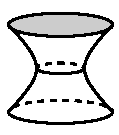
\includegraphics[scale=1.4]{hyperboloid1.pdf}} }
     & \raisebox{-48pt}[42pt][52pt]
              { \smash{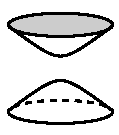
\includegraphics[scale=1.4]{hyperboloid2.pdf}} }
     & \raisebox{-46pt}[42pt][52pt]
              { \smash{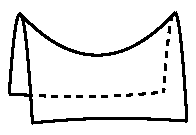
\includegraphics[scale=1.3]{hyperbolic_paraboloid.pdf}} }
      \\[0.1in]
  \hline
\end{tabular}






